\section{Search for a Kinematic Edge}
\label{sec:fit}

Many models of new physics produce an excess of same flavor (SF) $ee$ and $\mu\mu$ lepton pairs
with respect to opposite flavor (OF) $e\mu$ pairs. For example, such an excess occurs in SUSY models
in which the opposite-sign leptons are produced via the decay $\chi_2^0 \to \chi_1^0 \ell^+\ell^-$.
The kinematics of this decay also lead to a characteristic triangle-shaped feature in the distribution
of dilepton mass, which would provide unambiguous evidence for new physics.
In contrast, for the dominant background \ttbar, the flavors of the 2 leptons are uncorrelated,
as is also the case for other SM background processes such as $W^+W^-$ and DY$\to\tau^+\tau^-$.
Therefore, for these processes the rates of SF and OF lepton pairs are the same modulo differences
between the electron and muon selection efficiencies; 
furthermore, the kinematic properties of events containing SF and OF lepton pairs are the same. 
This allows us to determine the SM background in the SF final state using events in the OF
final state; this technique is referred to as OF subtraction. In Sec.~\ref{sec:datadriven}
we search for an excess of SF with respect to OF events accompanied by large \MET\ and \Ht. 
In this section, we perform a fit to search for a kinematic edge in the dilepton mass distribution 
in SF events, in which we extract the background shape from OF events.

In order to further suppress DY, we increase the \MET\ requirement to \MET $>$ 100 GeV. 
We search for the kinematic edge in 2 regions.  The first region is a control region defined
as 100 $<$ \Ht\ $<$ 300 GeV, which is dominated by the \ttbar\ background; we use 
this region to validate our fit methodology and verify that a signal yield consistent with 0 
is obtained. We then proceed to search for a kinematic edge in the signal region defined as 
\Ht\ $>$ 300 GeV. Since we do not observe a kinematic edge in this region, we perform a 
fit to the dilepton mass distribution assuming an example signal shape from the LM1 scenario.
The residual DY background in the control region is fitted and extrapolated
to the signal region where it is found to be very small.


In addition to the background shapes the yields in the $e\mu$, $ee$ and $\mu\mu$
channel are connected when correcting for the difference in lepton selection efficiencies
using $R_{\mu e} = 1.13 \pm 0.05$ (the ratio of muon to electron selection efficiencies),
evaluated by taking the square root of the ratio of the number of 
$Z \to \mu^+\mu^-$ to $Z \to e^+e^-$ events in data, in the mass range 76-106 GeV with no jets or 
\met\ requirements. 
 
The background as a function of the invariant mass $\mll$ is described by:

\begin{equation}
B(\mll) = \mll^a e^{-b \mll}.
\end{equation}

Its shape compared to the dilepton mass distribution in the control region
for events containing OF lepton pairs is shown in Fig.~\ref{fig:dilmass} (upper-right).

For a potential signal, we use an edge model for a two-body decay, 
which comprises a triangular shape convoluted with a gaussian,
according to:

\begin{equation}
T(\mll) = \frac{1}{\sqrt{2\pi}\sigma}\int_0^{M_{cut}} dy~y e^{\frac{(-(\mll-y)^2}{2\sigma^2}},
\end{equation}

where the resolution $\sigma$ is fixed based on simulation.

\begin{figure}[hbt]
\begin{center}
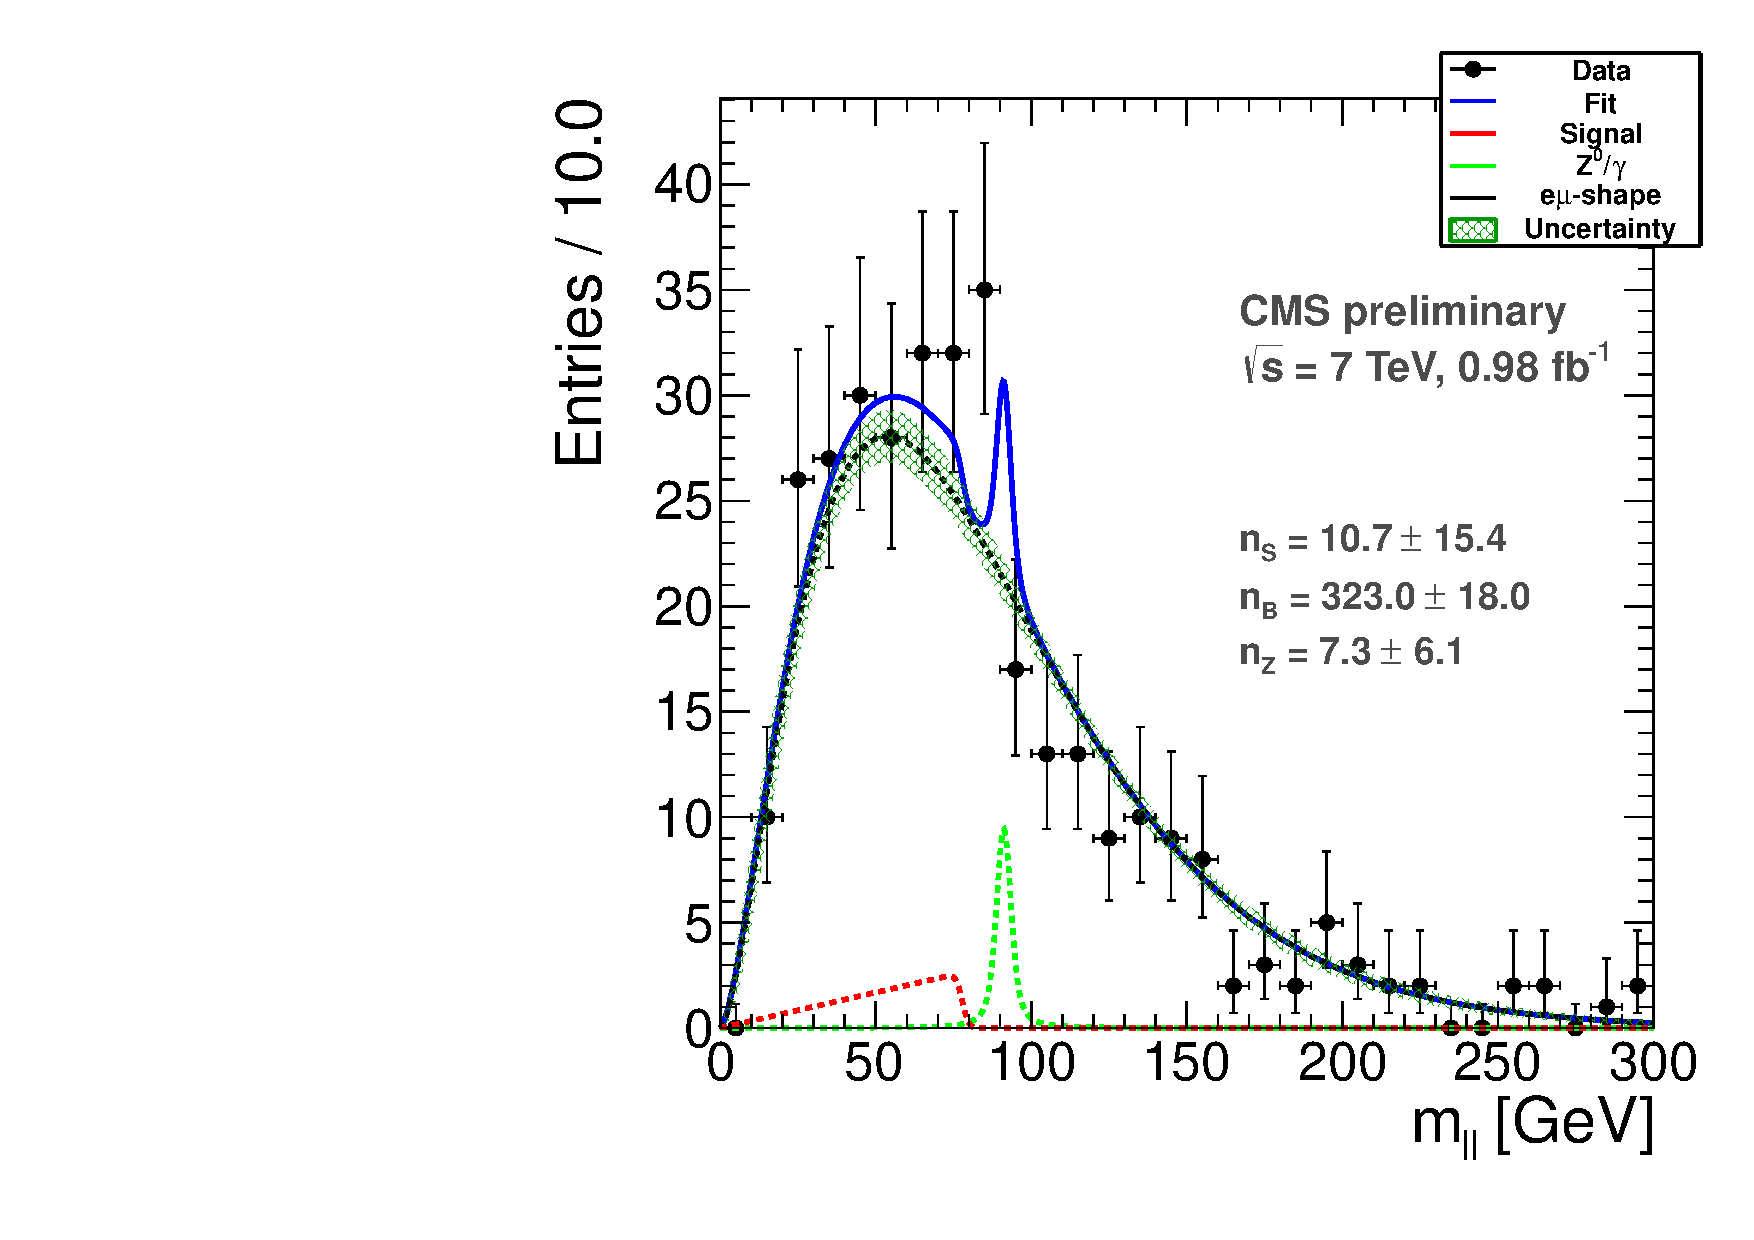
\includegraphics[width=0.48\linewidth]{plots_final/fit2011_Control_Data.pdf}
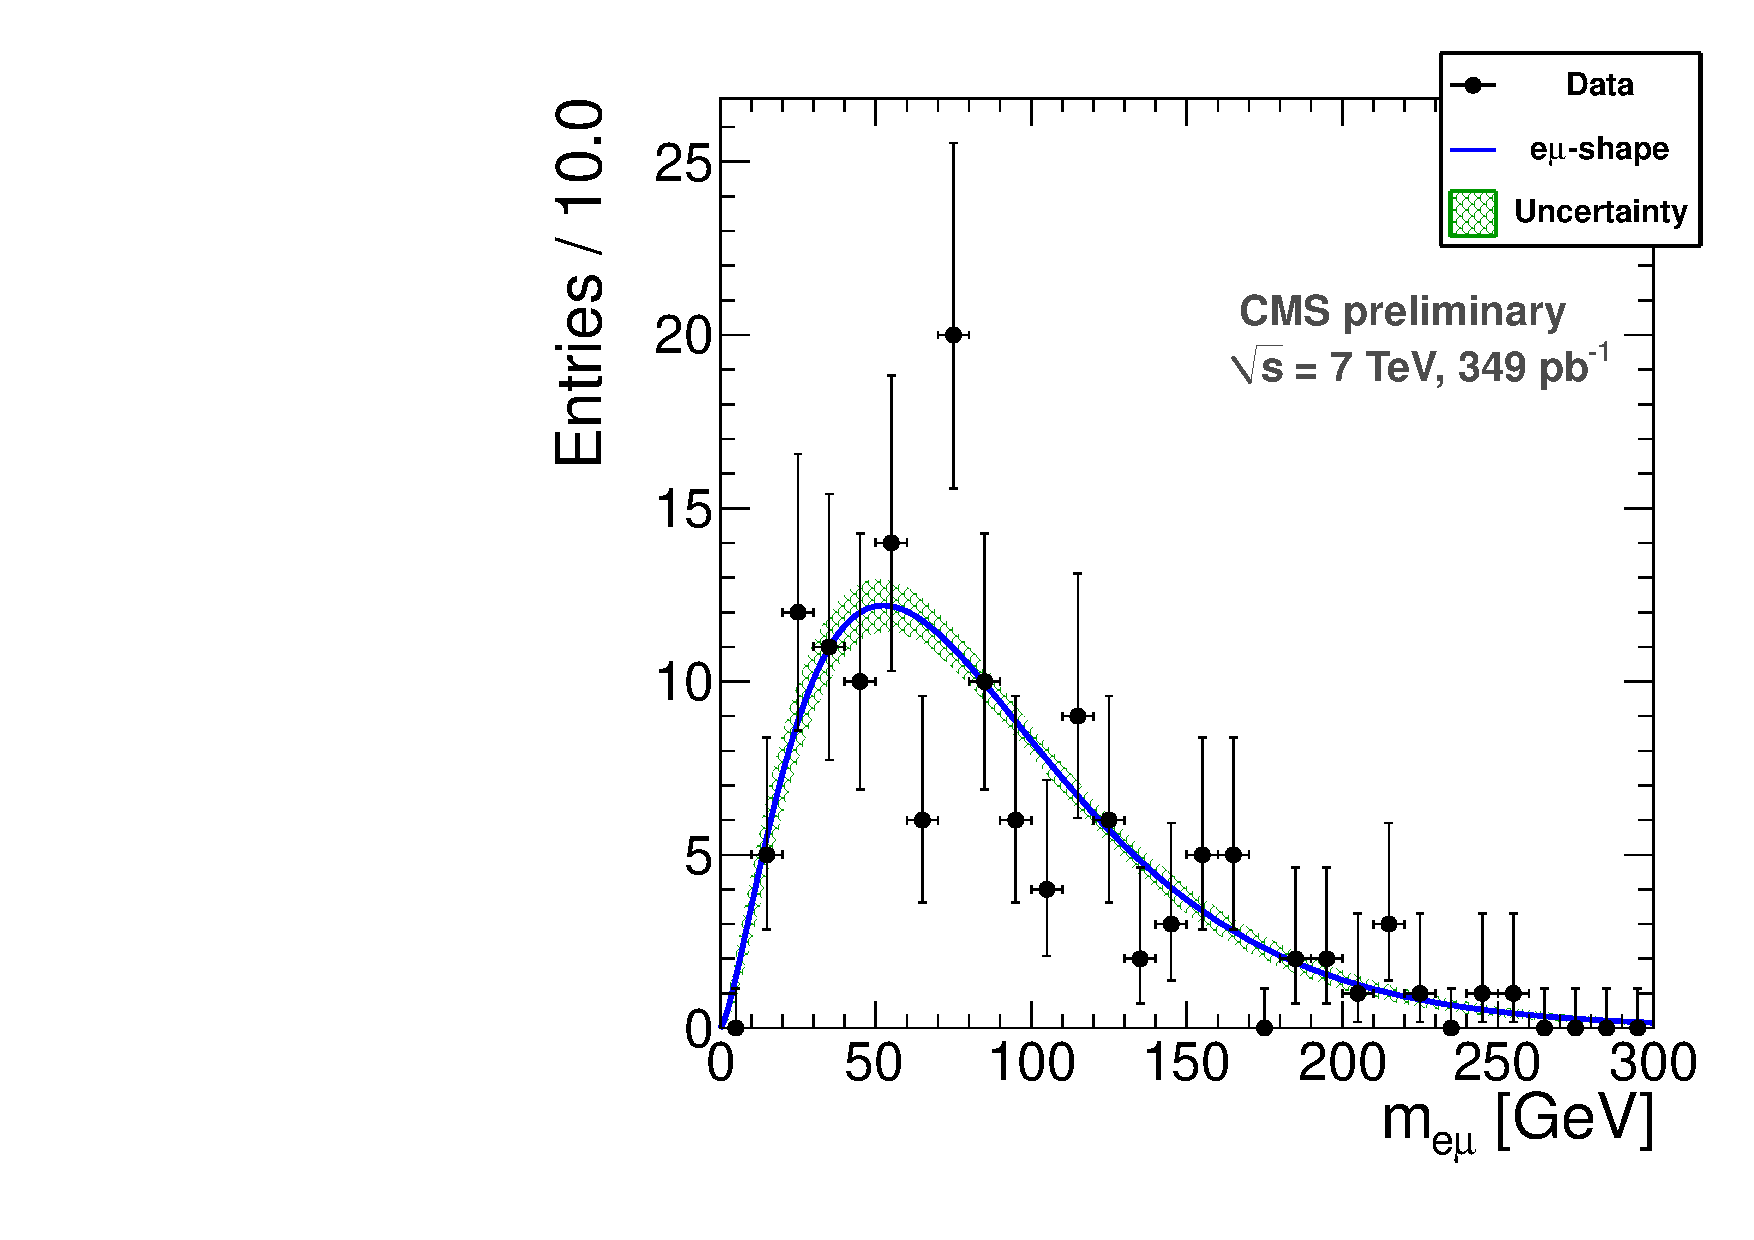
\includegraphics[width=0.48\linewidth]{plots_final/fit2011OFOS_Control_Data.pdf}
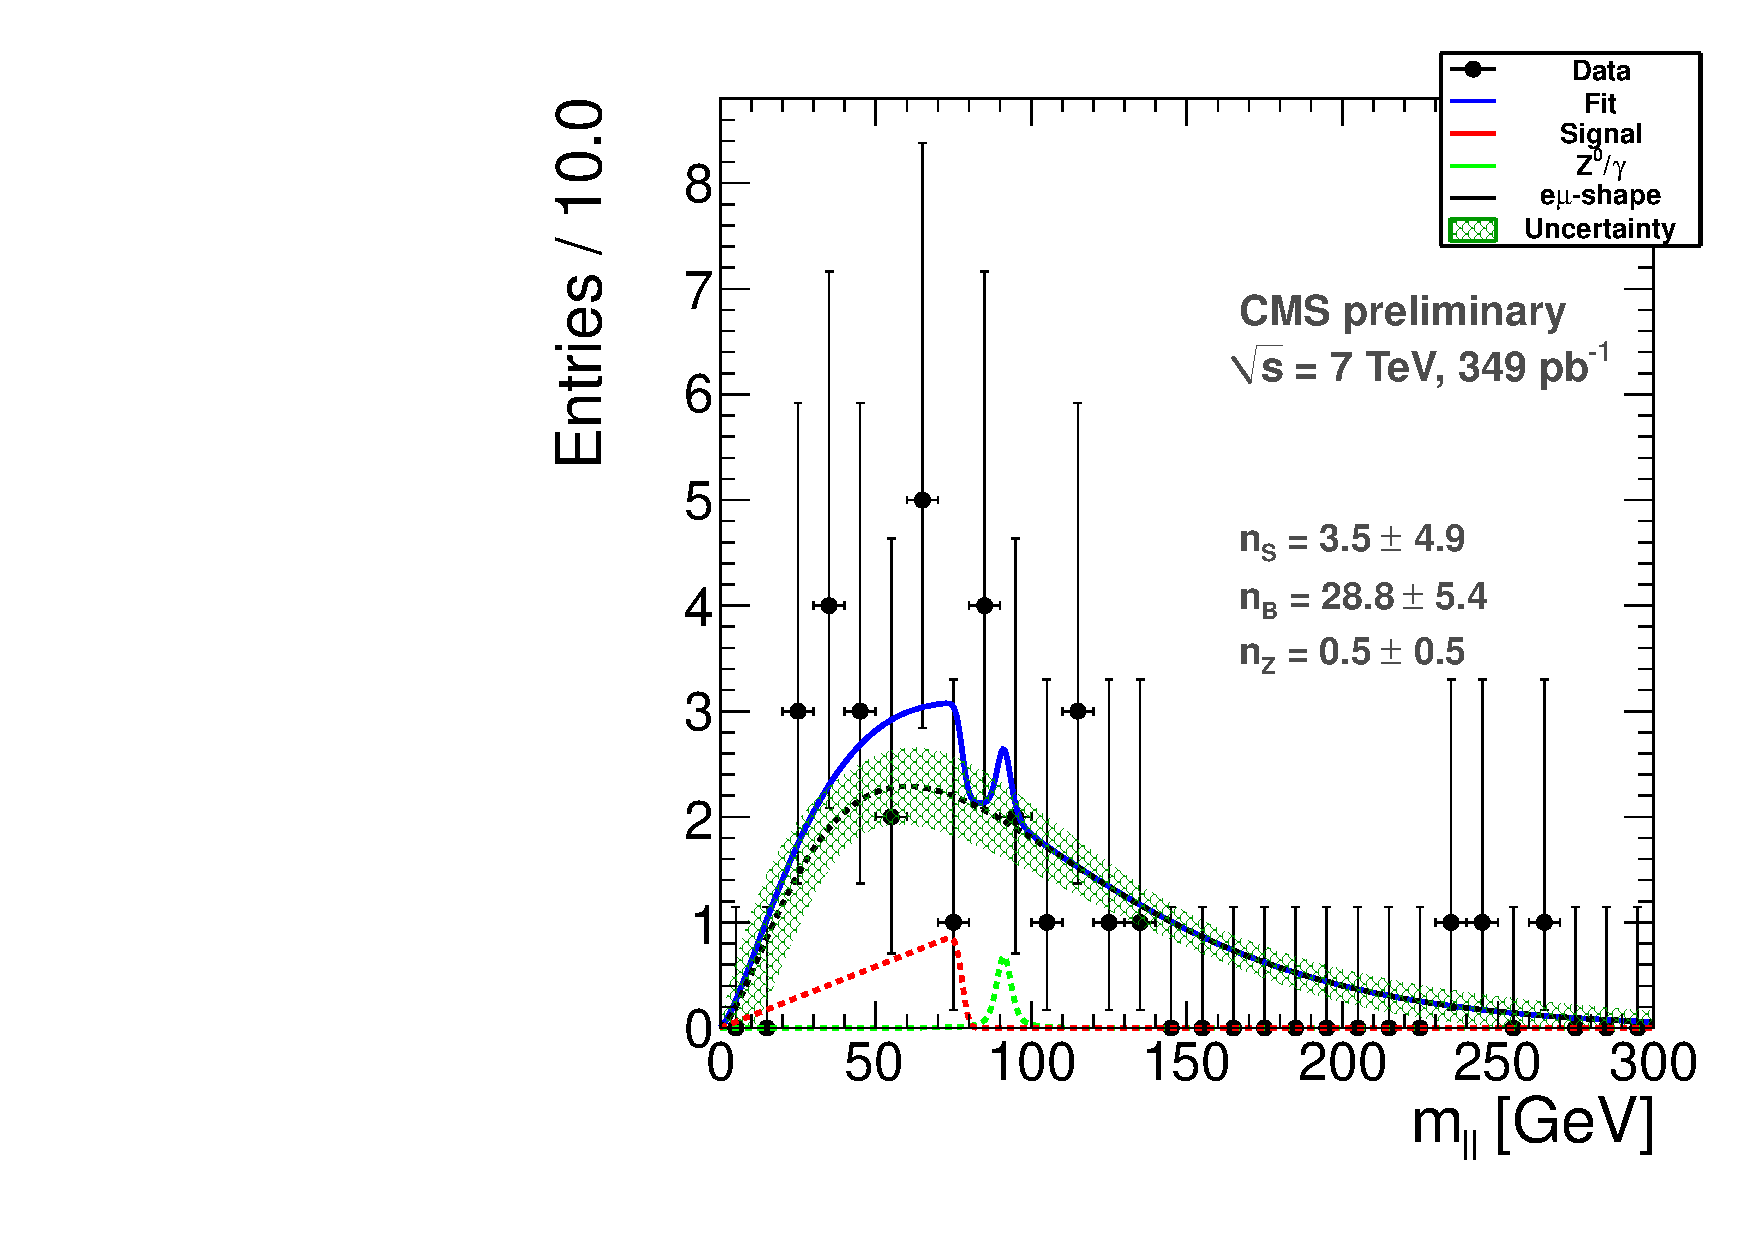
\includegraphics[width=0.48\linewidth]{plots_final/fit2011_Signal_Data.pdf}
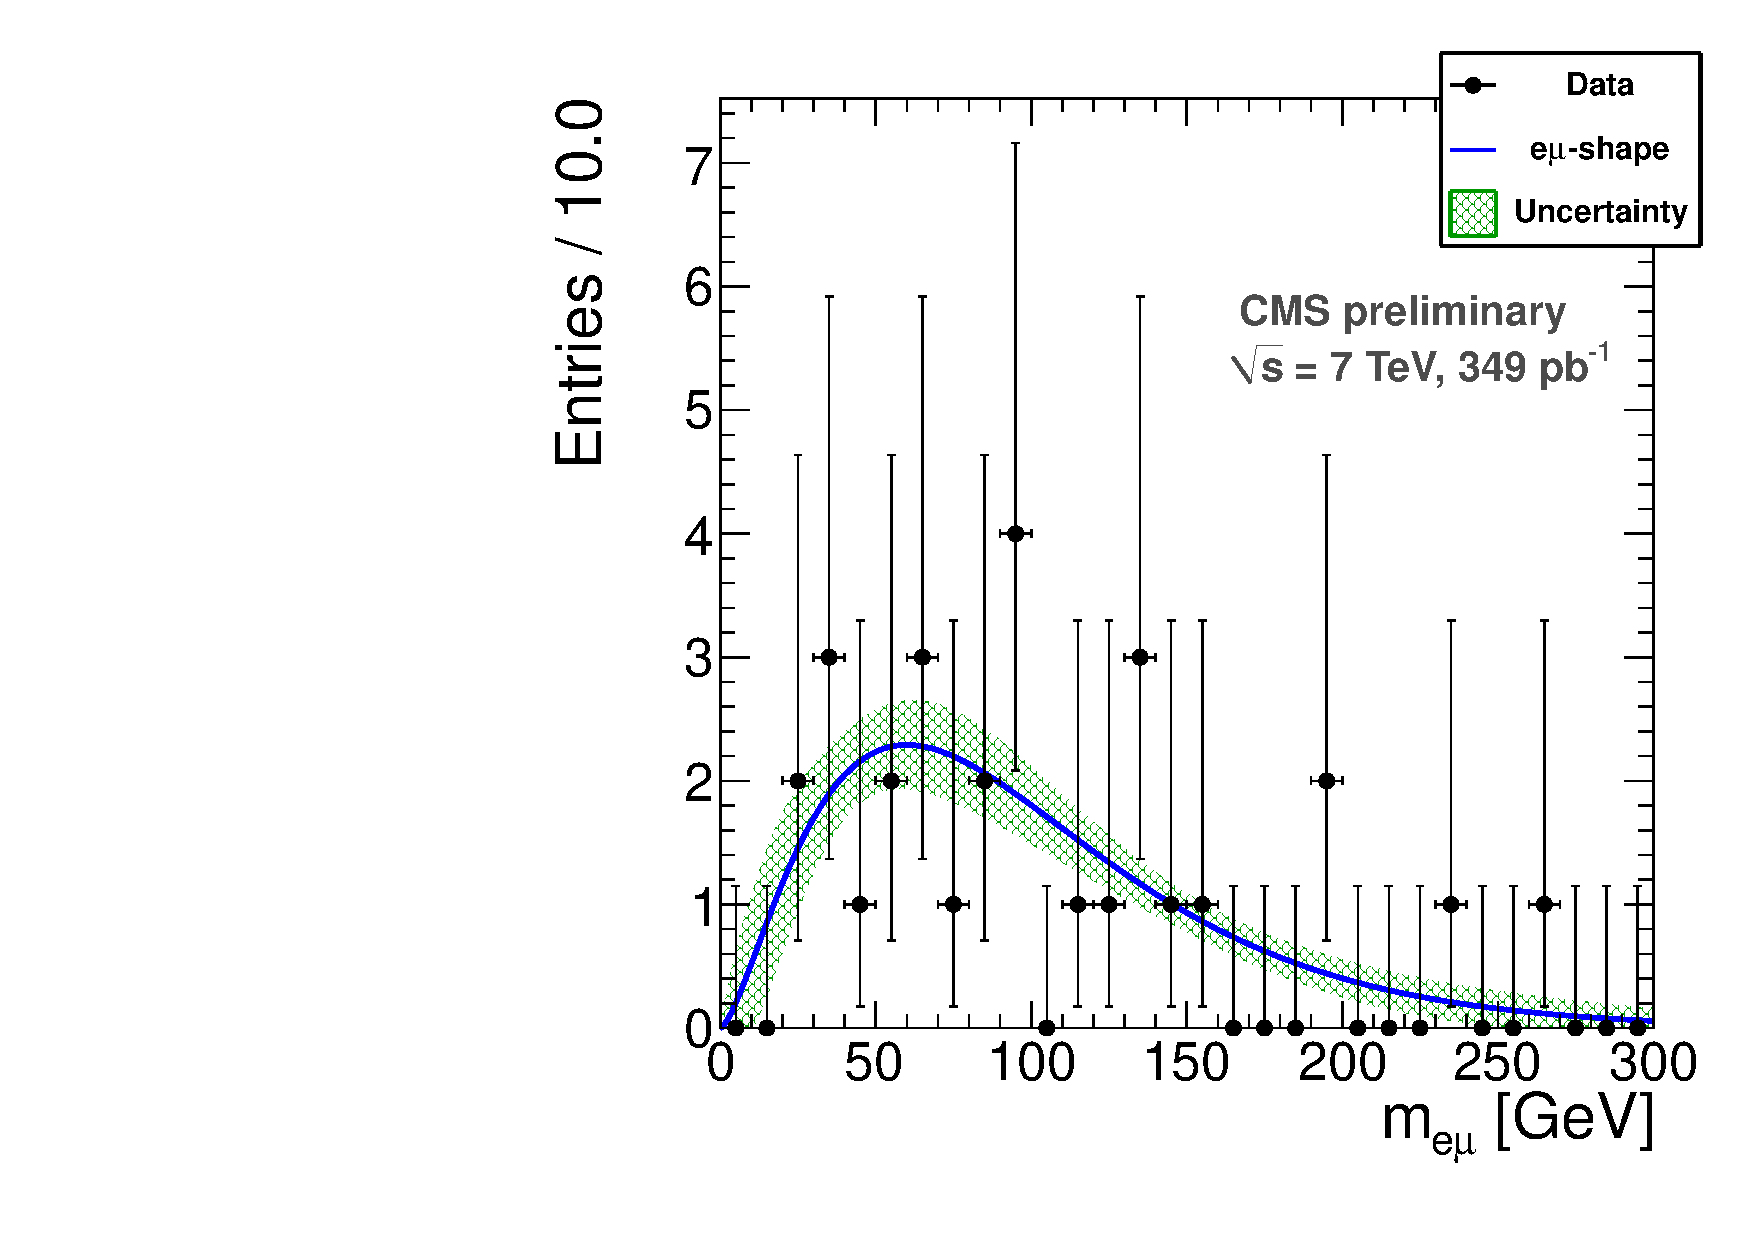
\includegraphics[width=0.48\linewidth]{plots_final/fit2011OFOS_Signal_Data.pdf}
\caption{\label{fig:dilmass}\protect 
Results of the maximum likelihood fit to the dilepton mass distribution for events containing 
$ee$ and $\mu\mu$ lepton pairs (left) and $e\mu$ lepton pairs (right) in the control
region defined as 100 $<$ \Ht\ $<$ 300~GeV, \MET\ $>$ 100 GeV (upper) and the signal region
\Ht\ $>$ 300~GeV, \MET\ $>$ 100 GeV (lower). In the extended fit the number of
signal $n_{S}$, Z $n_Z$ and \ttbar\ $n_B$ events is extracted as well.
}
\end{center}
\end{figure}

The position of the kinematic edge $M_{cut}$ is fixed based on the generator level
information for the signal model which is tested; for example, for LM1 
$M_{cut} = 77.8$~GeV. Finally, the $Z$ contribution is modelled by a Breit-Wigner 
convoluted with a Gaussian (with fixed Z mass and width). 

We perform a simultaneous, extended, unbinned maximum 
likelihood (ML) fit to the distribution of dilepton mass for events containing $ee$, $\mu\mu$ 
(signal, Z and background model)
and $e\mu$ pairs (background model only). 
The shape of the \ttbar\ background shape is assumed to be common in all categories
and the yields of signal $n_S$, Z $n_Z$ and background $n_B$ 
in the three categories are connected using $R_{\mu e}$. 

We perform the fit in the control region 100 $<$ \Ht\ $<$ 300 GeV, in
which the \ttbar\ background, $Z$ background, and LM1 signal yields are allowed to vary in the fit. 
The extracted signal yield is $n_S = 0.0 \pm 7.3$, consistent with the background only 
hypothesis, as displayed in Fig.~\ref{fig:dilmass} (upper-left). 
The extracted $Z$ yield is $n_Z = 5.2 \pm 4.2$, which is 
used to constrain the $Z$ yield in the signal region. 

Next, we perform the fit in the signal region \Ht\ $>$ 300 GeV. The \ttbar\ shape
overlaid for OF events, as shown in Fig.~\ref{fig:dilmass} (lower-right). We
constrain the $Z$ yield in this region using an extrapolation in \Ht\ from the 
control region 100 $<$ \Ht\ $<$ 300 GeV. The $Z$ yield in the control region is
multiplied by a scale factor derived from $Z$ events in data with no requirement
on \MET, which quantifies the fraction of $Z$ events with \Ht\ $>$ 100 GeV which 
satisfy \Ht\ $>$ 300 GeV. Using this procedure we derive an upper limit on the
$Z$ yield in the signal region of $n_Z < 0.3$, which we use to constrain the
$Z$ yield in the ML fit. The extracted signal yield is $n_S = 3.5 \pm 4.9$,
which is consistent with the background only hypothesis,
as shown in Fig.~\ref{fig:dilmass} (lower-left). 
